% (c) 2002 Matthew Boedicker <mboedick@mboedick.org> (original author) http://mboedick.org
% (c) 2003-2007 David J. Grant <davidgrant-at-gmail.com> http://www.davidgrant.ca
% (c) 2008 Nathaniel Johnston <nathaniel@nathanieljohnston.com> http://www.nathanieljohnston.com
% (c) 2011 Scott Clark <sc932@cornell.edu> http://cam.cornell.edu/~sc932
% (c) 2012 Arne Hassel <arne.hassel@gmail.com> http://megoth.wordpress.com/
%
%This work is licensed under the Creative Commons Attribution-Noncommercial-Share Alike 2.5 License. To view a copy of this license, visit http://creativecommons.org/licenses/by-nc-sa/2.5/ or send a letter to Creative Commons, 543 Howard Street, 5th Floor, San Francisco, California, 94105, USA.

\documentclass[letterpaper,11pt,english]{article}
\newlength{\outerbordwidth}
\pagestyle{empty}
\raggedbottom
\raggedright
\usepackage{babel}
\usepackage{float}
\usepackage[T1]{fontenc}
\usepackage{framed}
\usepackage{graphicx}
\usepackage[utf8]{inputenc}
\usepackage{tocloft}
\usepackage{url}
\usepackage[svgnames]{xcolor}
\usepackage{wrapfig}

%-----------------------------------------------------------

%Edit these values as you see fit

\setlength{\outerbordwidth}{3pt}  % Width of border outside of title bars
\definecolor{shadecolor}{gray}{0.75}  % Outer background color of title bars (0 = black, 1 = white)
\definecolor{shadecolorB}{gray}{0.93}  % Inner background color of title bars

%-----------------------------------------------------------

%Margin setup

\setlength{\evensidemargin}{-0.25in}
\setlength{\headheight}{-0.25in}
\setlength{\headsep}{0in}
\setlength{\oddsidemargin}{-0.25in}
\setlength{\paperheight}{11in}
\setlength{\paperwidth}{8.5in}
\setlength{\tabcolsep}{0in}
\setlength{\textheight}{9.75in}
\setlength{\textwidth}{7in}
\setlength{\topmargin}{-0.3in}
\setlength{\topskip}{0in}
\setlength{\voffset}{0.1in}

%-----------------------------------------------------------

%Custom commands

\newcommand{\resitem}[1]{\item #1 \vspace{-2pt}}

\newcommand{\resheading}[1]{\vspace{8pt}
  \parbox{\textwidth}{\setlength{\FrameSep}{\outerbordwidth}
    \begin{shaded}
\setlength{\fboxsep}{0pt}\framebox[\textwidth][l]{\setlength{\fboxsep}{4pt}\fcolorbox{shadecolorB}{shadecolorB}{\textbf{\sffamily{\mbox{~}\makebox[6.762in][l]{\large #1} \vphantom{p\^{E}}}}}}
    \end{shaded}
  }\vspace{-5pt}
}

\newcommand{\ressubheading}[4]{
\begin{tabular*}{6.5in}{l@{\cftdotfill{\cftsecdotsep}\extracolsep{\fill}}r}
		\textbf{#1} & #2 \\
		\textit{#3} & \textit{#4} \\
\end{tabular*}\vspace{-6pt}}

%-----------------------------------------------------------

\title{Curriculum Vitae}

\begin{document}

\begin{minipage}{\textwidth}
\begin{wrapfigure}{r}{0pt}
	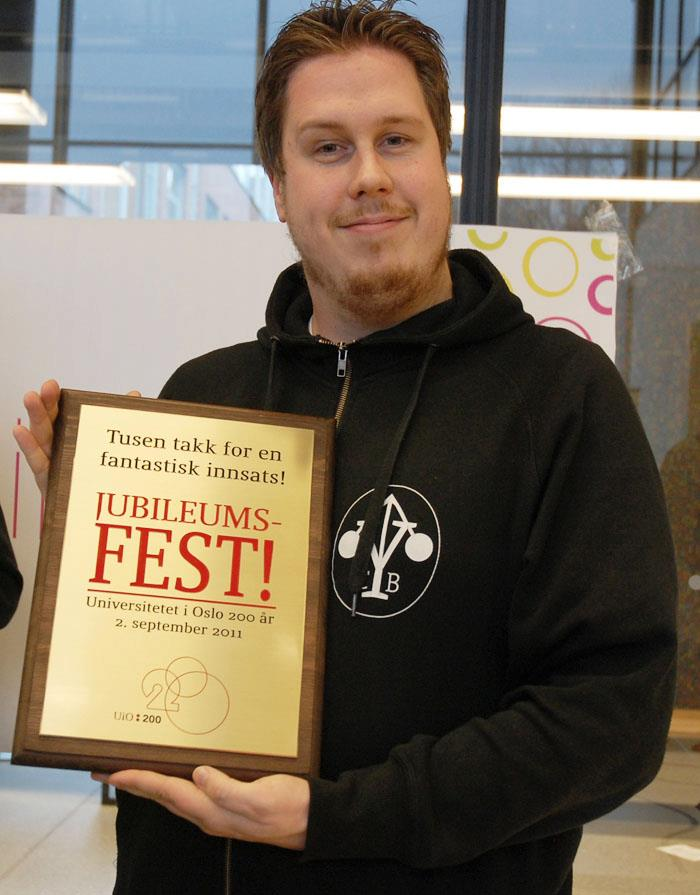
\includegraphics[height=45mm]{uio200.jpg}
\end{wrapfigure}

\textbf{\Large Curriculum Vitae for Arne Hassel}

\vspace{5mm}

\begin{tabular}{p{1in} l}
Adress: & Rosenborggata 15c, 0356 Oslo, NORWAY\\
Phone: & (+47) 416 94 086 \\
Mail: & \url{arne.hassel@gmail.com} \\
Born: & December 5th 1984 \\
Marital status: & Unmarried \\
\end{tabular}

\vspace{5mm}

\begin{minipage}{5.5in}
Soon to be graduated master in computer science, focused on webbased solutions. Experienced programmer, solution oriented and quick to learn new technologies and programming languages.
\end{minipage}

\end{minipage}

\resheading{Work Experience}

\begin{itemize}
\item
	\ressubheading{Centre for Shared Decision making and Collaborative Care Research}{Oslo, Norway}{System Developer}{2008 - current}
	\begin{itemize}
		\resitem{Work mostly frontend (HTML, CSS og Javascript),  but also some backend (.NET framework)}
	\end{itemize}
\item
	\ressubheading{Kiwi}{Risør \& Oslo, Norway}{Part-time worker}{1999 - 2008}
\item
	\ressubheading{Senter for Helse \& Arbeid}{Oslo, Norway}{Personal assistant}{2008}
\end{itemize}

\resheading{Education}
\begin{itemize}
\item
	\ressubheading{Department of informatics, University of Oslo}{Oslo, Norway}{Master in Computer Science: programming and networks (current)}{2010 - 2012 (estimated)}
	\begin{itemize}
		\item Working on my master thesis on Javascript and Semantic Web, my supervisors are Kjetil Kjernsmo and Martin Giese
		\item Programmed a lot in Java and Eclipse
	\end{itemize}
\item
	\ressubheading{Department of informatics, University of Oslo}{Oslo, Norway}{5-year Master, Distributed Systems and Networks}{2007 - 2010}
\item
	\ressubheading{Norwegian University of Life Sciences}{Ås, Norway}{Bachelor in Economics and Administration}{2003 - 2007}
\item
	\ressubheading{Risør VGS}{Risør, Norway}{General studies}{2000 - 2003}
\end{itemize}

\resheading{Skills}

See attached competence chart for more details.

\begin{itemize}
\item {\bf Development:} {\bf (Very good:)} CSS, HTML, Javascript, LESS, Sass, SQL, {\bf (Good:)} C\#, Java, PHP, Python, RDF, SPARQL, TTL, XML, XSLT, {\bf (Average:)} Assembly, C
\item {\bf Frameworks:} Compass, Django, .NET MVC 2 \& 3, Umbraco, Wordpress
\item {\bf Computer science:} Databases, semantic technologies, system development, algorithms, data structures, qualitative research, modeling, computer architecture, \LaTeX, design patterns
\item {\bf Administration:} Organizational analysis, SWOT-analysis, risk analysis
\item {\bf Economics:} Accounting, budgets, journaling, macro- \& microeconomics
\item {\bf Language:} Norwegian (native tongue), english (fluent)
\end{itemize}

\resheading{Selected projects}

\begin{itemize}
\item {\bf CommunicareTools:} Webpage focused on presenting the portfolio of Centre for Shared Decision making and Collaborative Care Research. Developed in .NET with the framework Umbraco. \url{http://communicaretools.org/}
\item {\bf Zetti:} A system to handle reports produced by Cybernetic Society. Developed in Django and Compass. Under development. \url{https://github.com/megoth/Zetti}
\end{itemize}

\resheading{Voluntary Work and Honorary Positions}

\begin{itemize}
\item
	\ressubheading{Cybernetic Society (CYB)}{Oslo, Norway}{Treasurer, Member of the Sponsor Board, Guard}{2009 - current}
	\begin{itemize}
		\resitem{Elected as Treasurer fall 2009 until spring 2011, now a resource person for the finance group.}
		\resitem{Helped stabilize the finances for CYB, so that the association could rise to become Institute Association, start maintaining a student pub, and become the largest association at the department.}
		\resitem{Administrated the work to publish Ifi-blekka 2011, an annual publication for the new students starting each fall.}
	\end{itemize}
\item
	\ressubheading{Birthday Party at Ole-Johan Dahls hus September 2nd}{Oslo, Norway}{Party General/Coordinator}{2011}
	\begin{itemize}
		\resitem{Planned, executed and completed the follow-up associated with the Birthday Party in the occasion of the 200-year celebration of University of Oslo.}
		\resitem{Cooperated with the department and UiO:200, the Anniversary Secreatariat, and executed a party for almost 5 000 people.}
	\end{itemize}
\item
	\ressubheading{IAESTE}{Ås, Norway}{Computer Manager, Leader, Treasurerer, Vice Leader}{2003 - 2007}
\item
	\ressubheading{UKA i Ås}{Ås, Norway}{Webmaster, Guard}{2004, 2006}
\end{itemize}

\resheading{Personal details}

\begin{itemize}
\item {\bf Hobbies:} Read, learn new stuff, build/create stuff (e.g. Lego), digital games, boardgames, cards and roleplaying-games.
\item Have a driver license class B (norwegian)
\end{itemize}

\resheading{References}

I will submit a list of my references if this would be appropriate.

\end{document}
